% Gabarit pandoc des corrigés publiés (brut et guidé). Contenu sans marque ni nom de site.
% Compilation : lualatex (latexmk -lualatex).
% Le Markdown reste la source unique : ne pas éditer ce fichier .tex à la main.
\documentclass[11pt,a4paper]{article}

% --- Moteur, polices (Latin Modern) et langue ---------------------------------
\usepackage{iftex}
\ifLuaTeX\else\errmessage{Ce document se compile avec lualatex}\fi
\usepackage{amsmath,amssymb,mathtools}
\usepackage{fontspec}
% mathrm=sym : \mathrm prend ses glyphes dans la police mathématique (ℓ, μ, Ω), comme KaTeX.
\usepackage[math-style=TeX,bold-style=TeX,mathrm=sym]{unicode-math}
% Repli pour les glyphes absents de Latin Modern (indices et exposants Unicode,
% flèches, filets des schémas en texte, symboles) : DejaVu, puis Latin Modern Math
% (ℓ, lettres mathématiques Unicode des légendes).
\directlua{
  luaotfload.add_fallback("repliTexte", {"DejaVuSerif:mode=harf;", "DejaVuSans:mode=harf;", "file:latinmodern-math.otf:mode=harf;"})
  luaotfload.add_fallback("repliMono", {"DejaVuSansMono:mode=harf;", "DejaVuSans:mode=harf;", "file:latinmodern-math.otf:mode=harf;"})
}
\setmainfont{Latin Modern Roman}[RawFeature={fallback=repliTexte}]
\setsansfont{Latin Modern Sans}[RawFeature={fallback=repliTexte}]
\setmonofont{Latin Modern Mono}[RawFeature={fallback=repliMono}]
\setmathfont{Latin Modern Math}
\usepackage[french]{babel}
\frenchsetup{SmallCapsFigTabCaptions=false}

% --- Mise en page --------------------------------------------------------------
\usepackage[a4paper,margin=2.2cm,headheight=14pt,footskip=1.2cm]{geometry}
\usepackage{microtype}
\setlength{\emergencystretch}{4em}
\tolerance=1500
\setlength{\parindent}{0pt}
\setlength{\parskip}{0.55\baselineskip plus 2pt minus 1pt}
\usepackage{xcolor}
% Gris nommés : babel-french rend « ! » actif dans le document.
\definecolor{gris2}{gray}{0.98}
\definecolor{gris3}{gray}{0.97}
\definecolor{gris5}{gray}{0.95}
\definecolor{gris35}{gray}{0.65}
\definecolor{gris40}{gray}{0.60}
\definecolor{gris45}{gray}{0.55}
\definecolor{gris50}{gray}{0.50}
\definecolor{gris55}{gray}{0.45}
\definecolor{gris60}{gray}{0.40}
\definecolor{gris65}{gray}{0.35}
\definecolor{gris70}{gray}{0.30}
\definecolor{gris80}{gray}{0.20}
\definecolor{gris85}{gray}{0.15}
\usepackage{graphicx}
\usepackage{float}
\usepackage{caption}
\captionsetup{font=small,labelformat=empty,justification=centering}
\usepackage{booktabs,longtable,array,multirow,calc}
\usepackage{siunitx}
\sisetup{locale=FR}
\usepackage[version=4]{mhchem}
\usepackage{listings}
\usepackage{fancyhdr}
\usepackage{lastpage}
\usepackage[most]{tcolorbox}
\usepackage{enumitem}
\setlist{nosep,leftmargin=*,topsep=2pt}
\usepackage[hidelinks,unicode]{hyperref}
\usepackage{bookmark}
\hypersetup{pdftitle={Centrale-Supélec MP — Physique-chimie 1 2026},pdfauthor={Rédigé par IA},pdfcreator={LaTeX},pdfsubject={Corrigé guidé}}
\usepackage{xurl}

% --- Pandoc : listes, tableaux, figures ----------------------------------------
\providecommand{\passthrough}[1]{#1}
\providecommand{\tightlist}{\setlength{\itemsep}{0pt}\setlength{\parskip}{0pt}}

\makeatletter
\def\maxwidth{\ifdim\Gin@nat@width>\linewidth\linewidth\else\Gin@nat@width\fi}
\def\maxheight{\ifdim\Gin@nat@height>0.55\textheight 0.55\textheight\else\Gin@nat@height\fi}
\makeatother
\setkeys{Gin}{width=\maxwidth,height=\maxheight,keepaspectratio}
\setcounter{secnumdepth}{-\maxdimen}
\providecommand{\pandocbounded}[1]{#1}
\usepackage{longtable,booktabs,array}

% --- Code (listings) -----------------------------------------------------------
\lstset{
  basicstyle=\ttfamily\small,
  columns=fullflexible,
  keepspaces=true,
  breaklines=true,
  breakatwhitespace=false,
  postbreak=\mbox{\textcolor{gris50}{$\hookrightarrow$}\space},
  frame=single,
  rulecolor=\color{gris35},
  framesep=4pt,
  xleftmargin=5pt,xrightmargin=5pt,
  backgroundcolor=\color{gris3},
  keywordstyle=\bfseries,
  commentstyle=\color{gris65},
  stringstyle=\color{gris80},
  showstringspaces=false,
  tabsize=4,
  extendedchars=true,
  aboveskip=6pt,belowskip=6pt,
}

% --- Macros des corrigés (KaTeX ↔ LaTeX) ---------------------------------------
% Les corrigés sont écrits pour KaTeX : on définit ici ce que KaTeX connaît et
% que LaTeX n'a pas, sans jamais retoucher le Markdown.
\providecommand{\R}{\mathbb{R}}
\providecommand{\N}{\mathbb{N}}
\providecommand{\Z}{\mathbb{Z}}
\providecommand{\Q}{\mathbb{Q}}
\providecommand{\C}{\mathbb{C}}
\providecommand{\dd}{\mathrm{d}}
\providecommand{\llbracket}{\lBrack}
\providecommand{\rrbracket}{\rBrack}
\providecommand{\lBrace}{\lbrace}
\providecommand{\rBrace}{\rbrace}
\providecommand{\Box}{\square}
\providecommand{\Diamond}{\lozenge}
\providecommand{\varnothing}{\emptyset}
\providecommand{\argmax}{\operatorname*{arg\,max}}
\providecommand{\argmin}{\operatorname*{arg\,min}}
\renewcommand{\leq}{\leqslant}
\renewcommand{\geq}{\geqslant}

% Équation hors texte : réduite à la largeur de la ligne si elle déborde.
\newsavebox{\boiteequation}
\newcommand{\equationajustee}[1]{%
  \sbox{\boiteequation}{$\displaystyle #1$}%
  \ifdim\wd\boiteequation>\linewidth
    \[\resizebox{\linewidth}{!}{\usebox{\boiteequation}}\]%
  \else
    \[#1\]%
  \fi}

% --- Encadrés pédagogiques (sobres, lisibles en noir et blanc) -----------------
\tcbset{
  encadre/.style={
    enhanced,breakable,sharp corners,
    colback=white,colframe=gris55,
    boxrule=0.4pt,leftrule=2.2pt,
    left=6pt,right=6pt,top=3pt,bottom=3pt,
    before skip=6pt,after skip=6pt,
    fonttitle=\bfseries\small,coltitle=black,
    attach title to upper,after title={\quad},
    parbox=false,
  }
}
\newtcolorbox{indication}[1]{encadre,colframe=gris45,colback=gris2,title={Indication~#1}}
\newtcolorbox{methode}{encadre,colframe=gris70,title={Méthode}}
\newtcolorbox{piege}{encadre,colframe=gris85,boxrule=0.8pt,leftrule=2.2pt,title={Piège}}
\newtcolorbox{jury}{encadre,colframe=gris60,colback=gris5,title={Jury}}
\newtcolorbox{encadrenote}{encadre,colframe=gris40}

% --- Titres de section ---------------------------------------------------------
\usepackage{titlesec}
\titleformat{\section}{\Large\bfseries}{}{0pt}{}
\titleformat{\subsection}{\large\bfseries}{}{0pt}{}
\titleformat{\subsubsection}{\normalsize\bfseries}{}{0pt}{}
\titlespacing*{\section}{0pt}{14pt plus 4pt minus 2pt}{6pt}
\titlespacing*{\subsection}{0pt}{10pt plus 3pt minus 2pt}{4pt}
\titlespacing*{\subsubsection}{0pt}{8pt plus 2pt minus 2pt}{2pt}

% --- En-tête et pied de page ---------------------------------------------------
\pagestyle{fancy}
\fancyhf{}
\fancyhead[L]{\small\textsc{Corrigé guidé} · Centrale-Supélec MP}
\fancyhead[R]{\small Physique-chimie 1 2026}
\fancyfoot[L]{\footnotesize Corrigé rédigé par IA, non officiel}
\fancyfoot[R]{\footnotesize \thepage\,/\,\pageref*{LastPage}}
\renewcommand{\headrulewidth}{0.4pt}
\renewcommand{\footrulewidth}{0pt}
\fancypagestyle{plain}{\fancyhf{}\fancyfoot[R]{\footnotesize \thepage\,/\,\pageref*{LastPage}}\fancyfoot[L]{\footnotesize Corrigé rédigé par IA, non officiel}\renewcommand{\headrulewidth}{0pt}}

\begin{document}
\thispagestyle{plain}
\begin{center}
  {\small\scshape Corrigé guidé}\par\smallskip
  {\LARGE\bfseries Centrale-Supélec MP — Physique-chimie 1 2026\par}\medskip
  {\large Centrale-Supélec · MP · Physique-chimie 1 · 2026\par}
\end{center}
\vspace{2pt}\hrule\vspace{8pt}

\emph{Corrigé rédigé par IA, non officiel. Signalez toute erreur.}

\hypertarget{pruxe9sentation-du-sujet}{%
\section{Présentation du sujet}\label{pruxe9sentation-du-sujet}}

\textbf{Format.} 4 heures, calculatrice autorisée, 46 questions (Q1 à Q46) réparties en trois parties « relativement indépendantes », sous le titre « Spectroscopie rovibrationnelle et laser ». Deux questions sont soulignées dans l'énoncé (prise d'initiative, barème valorisé) : \textbf{Q13} et \textbf{Q46}.

Un formulaire final rappelle l'identité \(\overrightarrow{\mathrm{rot}}\,\overrightarrow{\mathrm{rot}}=\overrightarrow{\mathrm{grad}}\,\mathrm{div}-\Delta\) et la relation de passage du champ électrique. Il donne aussi \(h\), \(c\) et la conversion \(1\ \mathrm{cm^{-1}}\leftrightarrow1{,}9863\times10^{-23}\ \mathrm J\).

Il fournit enfin les masses et abondances de \(^1\)H, \(^{35}\)Cl et \(^{37}\)Cl.

\textbf{Partie A --- Spectroscopie rovibrationnelle (Q1--Q14).}

\begin{itemize}
\tightlist
\item
  \emph{A.I (Q1--Q8)} : oscillateur harmonique classique (équation, énergies moyennes), puis quantique : énergies moyennes en fonction des écarts-types, énergie minimale imposée par Heisenberg, analyse dimensionnelle, équation de Schrödinger adimensionnée, équation d'Hermite et quantification \(E_n=(n+\frac12)\hbar\omega_0\).
\item
  \emph{A.II (Q9--Q14)} : rotateur rigide (\(E_J=BJ(J+1)\) donné), lecture d'un vrai spectre FTIR de HCl : branches P et R, attribution des raies, extinction des raies lointaines, mesure de \(d_0\) et \(\omega_0\) avec incertitudes, dédoublement isotopique.
\end{itemize}

\textbf{Partie B --- Cavité d'un laser (Q15--Q29).}

\begin{itemize}
\tightlist
\item
  \emph{B.I (Q15--Q19)} : équations de Maxwell, d'Alembert, relation de dispersion, conditions aux limites sur deux conducteurs parfaits, modes \(\nu_m=mc/2L\).
\item
  \emph{B.II (Q20--Q29)} : un miroir devient partiellement réfléchissant ; on construit l'onde intracavité par superposition, on obtient une fonction d'Airy, puis l'intervalle spectral libre, la finesse et l'intérêt d'une grande finesse en interférométrie.
\end{itemize}

\textbf{Partie C --- Milieu amplificateur (Q30--Q46).}

\begin{itemize}
\tightlist
\item
  \emph{C.I (Q30--Q35)} : cinétique d'ordre 1 d'un système à trois niveaux, conservation de la matière, inversion de population en régime stationnaire.
\item
  \emph{C.II (Q36--Q40)} : bilan local d'énergie électromagnétique dans une tranche de milieu, gain linéique et lien avec l'inversion.
\item
  \emph{C.III (Q41--Q46)} : exploitation d'un spectre réel de laser à colorant en microcavité (couleur, intervalle spectral libre en longueur d'onde, longueur de cavité, finesse, principe du capteur, spectre d'une cavité métrique).
\end{itemize}

\textbf{Notions du programme mobilisées.} Oscillateur harmonique ; introduction à la physique quantique (inégalité de Heisenberg, équation de Schrödinger, états stationnaires) ; analyse dimensionnelle ; incertitudes-types et propagation ; équations de Maxwell, ondes planes, réflexion sur un conducteur parfait, ondes stationnaires ; interférences à ondes multiples, cohérence temporelle ; cinétique chimique d'ordre 1 ; bilans locaux d'énergie (vecteur de Poynting) ; couleur et absorption.

\textbf{Difficulté et longueur.} Sujet long mais très progressif. Les points délicats sont Q3 (justifier \(\langle x\rangle=\langle p_x\rangle=0\)), Q10--Q11 (axe de la figure 3 orienté vers les nombres d'onde décroissants), Q13 (démarche et incertitudes), Q22--Q24 (signes et facteurs 2 de l'aller-retour), Q37 (bilan local proprement posé) et Q46 (question ouverte à chiffrer).

\textbf{Questions à ne pas laisser passer.} Q1, Q2, Q5--Q9, Q15--Q17, Q19, Q20, Q30--Q33, Q39, Q41 : du cours ou presque.

\textbf{Gestion du temps.} Environ 5 minutes par question. Viser 1 h 30 pour la partie A, 1 h pour la partie B, 1 h 30 pour la partie C. Les parties étant indépendantes, on peut commencer par B ou C si la mécanique quantique inquiète ; la partie C se termine sur des questions de lecture de figure rapides et rentables.

\begin{center}\rule{0.5\linewidth}{0.5pt}\end{center}

\hypertarget{partie-a-spectroscopie-rovibrationnelle}{%
\section{Partie A --- Spectroscopie rovibrationnelle}\label{partie-a-spectroscopie-rovibrationnelle}}

\hypertarget{i-vibration-de-hcl}{%
\subsection{I --- Vibration de HCl}\label{i-vibration-de-hcl}}

On compare l'oscillateur classique, qui peut être au repos, à l'oscillateur quantique, qui ne le peut pas. Outils : mécanique du point, inégalité de Heisenberg, équation de Schrödinger à une dimension.

\hypertarget{question-1}{%
\subsection{Question 1}\label{question-1}}

\begin{indication}{1}

Écrivez le principe fondamental de la dynamique avec la force qui dérive de \(E_p=\frac12\mu\omega_0^2x^2\).

\end{indication}

\begin{indication}{2}

« Solution générale » : deux constantes d'intégration.

\end{indication}

\hypertarget{solution}{%
\subsubsection{Solution}\label{solution}}

La force \(F_x=-\mathrm dE_p/\mathrm dx=-\mu\omega_0^2x\) et le PFD projeté sur \((Ox)\) (référentiel galiléen) donnent

\equationajustee{\boxed{\ddot x+\omega_0^2x=0}}

Les racines caractéristiques sont \(\pm j\omega_0\), d'où la solution générale

\equationajustee{\boxed{\begin{aligned}
x(t)&=A\cos(\omega_0t)+B\sin(\omega_0t)\\
&=X_m\cos(\omega_0t+\varphi)
\end{aligned}}}

avec deux constantes réelles fixées par les conditions initiales.

\begin{piege}

Donner seulement \(x=X_m\cos\omega_0t\) n'est pas la solution générale : il manque la phase (ou la seconde constante).

\end{piege}

\hypertarget{question-2}{%
\subsection{Question 2}\label{question-2}}

\begin{indication}{1}

Calculez les moyennes temporelles de \(E_c\) et \(E_p\) sur une période pour la solution de Q1.

\end{indication}

\begin{indication}{2}

Une valeur minimale doit être \emph{atteinte} : cherchez un mouvement classique qui l'atteint.

\end{indication}

\hypertarget{solution-1}{%
\subsubsection{Solution}\label{solution-1}}

Avec \(x=X_m\cos(\omega_0t+\varphi)\) et \(\langle\cos^2\rangle=\langle\sin^2\rangle=\frac12\) :

\equationajustee{\begin{aligned}
\langle E_c\rangle&=\tfrac14\mu\omega_0^2X_m^2\\
\langle E_p\rangle&=\tfrac14\mu\omega_0^2X_m^2\\
\langle E_m\rangle&=\tfrac12\mu\omega_0^2X_m^2
\end{aligned}}

Ces trois quantités sont positives et s'annulent pour \(X_m=0\), c'est-à-dire pour la particule au repos en \(x=0\), mouvement permis. \textbf{Les trois minima sont nuls et atteints.}

\begin{methode}

Pour un minimum, deux étapes : une minoration, puis un cas d'égalité réalisable.

\end{methode}

\hypertarget{question-3}{%
\subsection{Question 3}\label{question-3}}

\begin{indication}{1}

Partez de la définition de la variance : \(\Delta x^2=\langle x^2\rangle-\langle x\rangle^2\). Que faut-il établir sur \(\langle x\rangle\) et \(\langle p_x\rangle\) ?

\end{indication}

\begin{indication}{2}

Parité du potentiel pour \(\langle x\rangle\) ; fonction d'onde stationnaire réelle et nulle à l'infini pour \(\langle p_x\rangle\).

\end{indication}

\hypertarget{solution-2}{%
\subsubsection{Solution}\label{solution-2}}

Dans un état stationnaire lié, \(\lvert\Psi\rvert^2=\lvert\varphi(x)\rvert^2\), avec \(\varphi\to0\) à l'infini.

\emph{Position.} \(E_p\) est paire : si \(\varphi(x)\) est solution d'énergie \(E\), \(\varphi(-x)\) aussi.

Les états liés à une dimension étant non dégénérés, \(\varphi(-x)=\pm\varphi(x)\). Donc \(\lvert\varphi\rvert^2\) est paire :

\equationajustee{\begin{aligned}
\langle x\rangle&=0\\
\Delta x^2&=\langle x^2\rangle
\end{aligned}}

\emph{Quantité de mouvement.} On peut choisir \(\varphi\) réelle (équation à coefficients réels). Alors

\equationajustee{\begin{aligned}
\langle p_x\rangle&=-j\hbar\int\varphi\varphi'\,\mathrm dx\\
&=-j\hbar[\varphi^2/2]_{-\infty}^{+\infty}\\
&=0
\end{aligned}}

donc \(\Delta p_x^2=\langle p_x^2\rangle\).

D'où \(\langle E_p\rangle=\frac12\mu\omega_0^2\Delta x^2\) et \(\langle E_c\rangle=\Delta p_x^2/(2\mu)\) :

\equationajustee{\boxed{\begin{aligned}
K_1&=\tfrac12\mu\omega_0^2\\
K_2&=\frac1{2\mu}
\end{aligned}}}

\begin{piege}

\(\langle E_c\rangle\) fait intervenir \(\langle p_x^2\rangle\), pas \(\langle p_x\rangle^2\). Sans la justification \(\langle x\rangle=\langle p_x\rangle=0\), le remplacement de \(\langle x^2\rangle\) par \(\Delta x^2\) n'est pas fondé.

\end{piege}

\hypertarget{question-4}{%
\subsection{Question 4}\label{question-4}}

\begin{indication}{1}

Additionnez les deux énergies de Q3 et éliminez \(\Delta p_x\) à l'aide de l'inégalité de Heisenberg.

\end{indication}

\begin{indication}{2}

Il reste une fonction de \(\Delta x^2\) de la forme \(a/X+bX\) : minorez-la (dérivée ou inégalité arithmético-\allowbreak{}géométrique).

\end{indication}

\hypertarget{solution-3}{%
\subsubsection{Solution}\label{solution-3}}

\(\langle E_m\rangle=\dfrac{\Delta p_x^2}{2\mu}+\dfrac12\mu\omega_0^2\Delta x^2\) et \(\Delta p_x\ge\hbar/(2\Delta x)\) donnent

\equationajustee{\begin{aligned}
\langle E_m\rangle&\ge\frac{\hbar^2}{8\mu\Delta x^2}+\frac12\mu\omega_0^2\Delta x^2\\
&\ge2\sqrt{\frac{\hbar^2}{8\mu}\cdot\frac{\mu\omega_0^2}{2}}\\
&=\frac{\hbar\omega_0}{2}
\end{aligned}}

avec égalité pour \(\Delta x^2=\hbar/(2\mu\omega_0)\) :

\equationajustee{\boxed{\langle E_m\rangle_{\min}=\frac{\hbar\omega_0}{2}}}

Classiquement, le minimum est nul. Quantiquement, localiser parfaitement la particule au fond du puits (\(\Delta x=0\)) rendrait \(\Delta p_x\) infini : le compromis laisse une \textbf{énergie de point zéro} \(\hbar\omega_0/2\), qui est l'énergie du niveau fondamental (Q8).

\begin{piege}

L'inégalité de Heisenberg donne une \emph{minoration} de \(\Delta p_x\), donc de \(\langle E_c\rangle\). Il faut ensuite minimiser sur \(\Delta x\), et non évaluer en une valeur arbitraire.

\end{piege}

\hypertarget{question-5}{%
\subsection{Question 5}\label{question-5}}

\begin{indication}{1}

Écrivez les dimensions de \(\hbar\), \(\omega_0\), \(\mu\) en masse, longueur, temps, puis identifiez les exposants.

\end{indication}

\hypertarget{solution-4}{%
\subsubsection{Solution}\label{solution-4}}

Les dimensions sont \([\hbar]=\mathrm{M\,L^2\,T^{-1}}\), \([\omega_0]=\mathrm T^{-1}\) et \([\mu]=\mathrm M\). L'égalité \([a_0]=\mathrm L\) impose :

\equationajustee{\begin{aligned}
\alpha+\delta&=0\\
2\alpha&=1\\
\alpha+\beta&=0
\end{aligned}}

\equationajustee{\boxed{\begin{aligned}
\alpha&=\tfrac12\\
\beta&=-\tfrac12\\
\delta&=-\tfrac12
\end{aligned}}}

\equationajustee{\boxed{a_0=\sqrt{\frac{\hbar}{\mu\omega_0}}}}

Avec \(\mu\simeq1{,}66\times10^{-27}\) kg et \(\omega_0\simeq10^{15}\) rad·s⁻¹ :

\equationajustee{\boxed{a_0\approx8\times10^{-12}\ \mathrm m\sim10^{-11}\ \mathrm m}}

soit quelques pour cent de la longueur de liaison : les oscillations sont petites, le modèle harmonique est cohérent.

\begin{piege}

\(\hbar\) contient une masse : \([\hbar]=\mathrm{J\cdot s}=\mathrm{kg\,m^2\,s^{-1}}\). Contrôle : \(\hbar\omega\) est une énergie.

\end{piege}

\hypertarget{question-6}{%
\subsection{Question 6}\label{question-6}}

\begin{indication}{1}

Séparez les variables dans l'équation de Schrödinger dépendante du temps : la partie temporelle d'un état stationnaire est une exponentielle.

\end{indication}

\begin{indication}{2}

Pour le changement de variable, \(\mathrm d^2/\mathrm dx^2=a_0^{-2}\,\mathrm d^2/\mathrm du^2\), puis calculez les deux préfacteurs avec \(a_0^2=\hbar/(\mu\omega_0)\).

\end{indication}

\hypertarget{solution-5}{%
\subsubsection{Solution}\label{solution-5}}

\equationajustee{\boxed{\chi(t)=\chi_0\,e^{-jEt/\hbar}}}

La partie spatiale vérifie

\equationajustee{-\frac{\hbar^2}{2\mu}\varphi_{xx}+\frac12\mu\omega_0^2x^2\varphi=E\varphi}

Avec \(x=a_0u\), les deux préfacteurs valent

\equationajustee{\begin{aligned}
\frac{\hbar^2}{2\mu a_0^2}&=\frac{\hbar\omega_0}{2}\\
\frac12\mu\omega_0^2a_0^2&=\frac{\hbar\omega_0}{2}
\end{aligned}}

En divisant par \(\hbar\omega_0\) :

\equationajustee{\boxed{\varphi''(u)+\left(2\varepsilon-u^2\right)\varphi(u)=0}}

\begin{piege}

Le signe de l'exponentielle temporelle se contrôle en reportant dans \(j\hbar\,\partial_t\Psi=E\Psi\) : c'est \(e^{-jEt/\hbar}\).

\end{piege}

\hypertarget{question-7}{%
\subsection{Question 7}\label{question-7}}

\begin{indication}{1}

Dérivez deux fois le produit \(\mathcal H(u)e^{-u^2/2}\) et reportez dans l'équation de Q6.

\end{indication}

\hypertarget{solution-6}{%
\subsubsection{Solution}\label{solution-6}}

\equationajustee{\begin{aligned}
\varphi'&=(\mathcal H'-u\mathcal H)e^{-u^2/2}\\
\varphi''&=\left(\mathcal H''-2u\mathcal H'+(u^2-1)\mathcal H\right)e^{-u^2/2}
\end{aligned}}

En reportant, puis en simplifiant par \(e^{-u^2/2}\neq0\) (les termes en \(u^2\mathcal H\) se compensent) :

\equationajustee{\boxed{\mathcal H''-2u\mathcal H'+(2\varepsilon-1)\mathcal H=0}}

\hypertarget{question-8}{%
\subsection{Question 8}\label{question-8}}

\begin{indication}{1}

Quel est le degré de chacun des trois termes ? Identifiez le coefficient de \(u^n\).

\end{indication}

\hypertarget{solution-7}{%
\subsubsection{Solution}\label{solution-7}}

\(\mathcal H''\) est de degré \(n-2\). Le coefficient de \(u^n\) doit être nul, avec \(c_n\neq0\) :

\equationajustee{-2nc_n+(2\varepsilon-1)c_n=0}

\equationajustee{\boxed{\varepsilon=n+\tfrac12}}

d'où

\equationajustee{\boxed{E_n=\left(n+\tfrac12\right)\hbar\omega_0,\ n\in\mathbb N}}

Niveaux équidistants de \(\hbar\omega_0\) ; le fondamental sature la borne de Q4.

\begin{figure}[H]
\centering
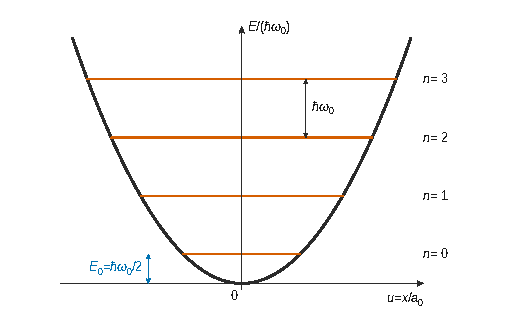
\includegraphics{figures/q8-niveaux-oscillateur.pdf}
\caption*{Figure 1 --- Puits harmonique et niveaux E\_n = (n + ½)ħω₀ : niveaux
équidistants de ħω₀, fondamental à l'énergie de point zéro ħω₀/2}
\end{figure}

\begin{methode}

Chercher une solution polynomiale d'une équation différentielle linéaire : le terme de plus haut degré donne une condition (ici la quantification), les autres une récurrence sur les coefficients.

\end{methode}

\hypertarget{ii-rovibration-de-hcl}{%
\subsection{II --- Rovibration de HCl}\label{ii-rovibration-de-hcl}}

On ajoute la rotation et on confronte le modèle à un spectre réel. Outils : lecture de figure, modélisation linéaire, incertitudes-types.

\hypertarget{question-9}{%
\subsection{Question 9}\label{question-9}}

\begin{indication}{1}

Développez et factorisez par \((J+1)\).

\end{indication}

\hypertarget{solution-8}{%
\subsubsection{Solution}\label{solution-8}}

\equationajustee{\begin{aligned}
\Delta E_J&=B\left[(J+1)(J+2)-J(J+1)\right]\\
&=\boxed{2B(J+1)}
\end{aligned}}

Les niveaux de rotation ne sont pas équidistants, contrairement aux niveaux de vibration.

\hypertarget{question-10}{%
\subsection{Question 10}\label{question-10}}

\begin{indication}{1}

Écrivez l'énergie d'une transition \((n=0,J'')\to(n=1,J')\) dans les deux cas \(\Delta J=\pm1\) et comparez-la à \(\hbar\omega_0\).

\end{indication}

\begin{indication}{2}

Regardez le sens de l'axe de la figure 3 et cherchez l'endroit où l'espacement entre raies est anormal.

\end{indication}

\hypertarget{solution-9}{%
\subsubsection{Solution}\label{solution-9}}

Avec \(\tilde B=B/hc\) et \(\tilde\nu_0=\omega_0/(2\pi c)\) :

\begin{itemize}
\tightlist
\item
  branche R (\(J'=J''+1\)) : \(\tilde\nu=\tilde\nu_0+2\tilde B(J''+1)\), au-dessus du centre ;
\item
  branche P (\(J'=J''-1\)) : \(\tilde\nu=\tilde\nu_0-2\tilde BJ''\), en dessous.
\end{itemize}

Les raies sont espacées d'environ 20 cm⁻¹, sauf entre 2865 et 2906 cm⁻¹ (41 cm⁻¹, soit \(4\tilde B\)).

Ce trou est le centre de bande, \(\tilde\nu_0\approx2886\) cm⁻¹, où \(\Delta J=0\) est interdit. On en déduit :

\equationajustee{\boxed{\begin{aligned}{}&\text{R : }[2886\,;3100]\ \mathrm{cm^{-1}}\ (\text{raies de 2906 \text{à} 3073})\\
&\text{P : }[2600\,;2886]\ \mathrm{cm^{-1}}\ (\text{raies de 2626 \text{à} 2865})
\end{aligned}}}

\begin{figure}[H]
\centering
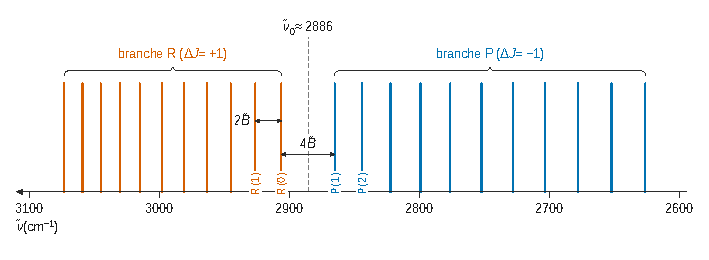
\includegraphics{figures/q10-branches-p-r.pdf}
\caption*{Figure 2 --- Lecture de la figure 3 (axe décroissant) : branche R à
gauche, branche P à droite, trou central de 4B̃ autour de ν̃₀ ≈ 2886 cm⁻¹,
attribution de R(0), R(1), P(1) et P(2)}
\end{figure}

\begin{piege}

L'axe de la figure 3 est gradué de 3100 à 2600 cm⁻¹ : la branche R, de plus haute énergie, est à \emph{gauche}.

\end{piege}

\hypertarget{question-11}{%
\subsection{Question 11}\label{question-11}}

\begin{indication}{1}

Numérotez les raies à partir du trou central, de part et d'autre.

\end{indication}

\begin{indication}{2}

La branche P n'a pas de raie P(0).

\end{indication}

\hypertarget{solution-10}{%
\subsubsection{Solution}\label{solution-10}}

\begin{longtable}[]{@{}llll@{}}
\toprule\noalign{}
\(\tilde\nu\) (cm⁻¹) & \(J''\) & \(J'\) & branche \\
\midrule\noalign{}
\endhead
\bottomrule\noalign{}
\endlastfoot
2926 & 1 & 2 & R \\
2906 & 0 & 1 & R \\
2865 & 1 & 0 & P \\
2844 & 2 & 1 & P \\
\end{longtable}

Contrôle avec \(\tilde\nu_0=2885{,}5\) et \(\tilde B=10{,}25\) cm⁻¹ : 2906 ; 2926,5 ; 2865 ; 2844,5 cm⁻¹, conforme à l'incertitude de lecture.

\begin{piege}

\(J''\) est le niveau de \emph{départ} (état fondamental), \(J'\) le niveau d'\emph{arrivée}. Oublier l'absence de P(0) décale toute la branche P d'une unité.

\end{piege}

\hypertarget{question-12}{%
\subsection{Question 12}\label{question-12}}

\begin{indication}{1}

Les règles de sélection autorisent des raies pour tout \(J''\) : qu'est-ce qui pourrait néanmoins les rendre invisibles ?

\end{indication}

\begin{indication}{2}

L'intensité d'une raie d'absorption dépend du nombre de molécules dans le niveau de départ. Comparez \(BJ''(J''+1)\) à \(k_BT\) à température ambiante, en cm⁻¹.

\end{indication}

\hypertarget{solution-11}{%
\subsubsection{Solution}\label{solution-11}}

Les raies de la bande \(0\to1\) s'éloignent du centre de \(2\tilde B\) par unité de \(J''\). Les autres transitions (rotation pure à quelques dizaines de cm⁻¹, bande \(0\to2\) vers 5800 cm⁻¹) tombent loin de la fenêtre.

L'intensité d'une raie est proportionnelle à la population du niveau \(J''\), pondérée par \(\exp\left(-\tilde BJ''(J''+1)hc/k_BT\right)\). À 300 K, \(k_BT/hc\approx208\) cm⁻¹.

Ce facteur vaut \(4\times10^{-3}\) pour \(J''=10\). Il tombe à \(5\times10^{-4}\) pour \(J''=12\).

Les raies qui tomberaient hors de \(2886\pm250\) cm⁻¹ partent de niveaux quasi vides : \textbf{aucune transition permise issue d'un niveau peuplé n'existe hors de \([2600\,;3100]\) cm⁻¹.}

\begin{piege}

« Les règles de sélection l'interdisent » est faux : \(\Delta J=\pm1\) est possible quel que soit \(J''\). C'est la population thermique qui éteint les raies.

\end{piege}

\hypertarget{question-13}{%
\subsection{Question 13}\label{question-13}}

\begin{indication}{1}

Question à initiative : choisissez les raies à exploiter et justifiez ce choix. Deux inconnues (\(\tilde\nu_0\), \(\tilde B\)) : deux raies bien choisies suffisent.

\end{indication}

\begin{indication}{2}

Les deux raies qui encadrent le trou central donnent directement une somme et une différence. Propagez les incertitudes-types (somme quadratique), puis passez à \(d_0\) par \(B=\hbar^2/(2\mu d_0^2)\) avec la \emph{masse réduite}.

\end{indication}

\begin{indication}{3}

\(\hbar\omega_0\) est l'écart entre niveaux vibrationnels, donc l'énergie du centre de bande.

\end{indication}

\hypertarget{solution-12}{%
\subsubsection{Solution}\label{solution-12}}

\emph{Démarche.} R(0) et P(1) sont les raies de plus petit \(J\), donc les moins sensibles à la différence des constantes rotationnelles entre les deux états :

\equationajustee{\begin{aligned}
\tilde\nu_0&=\frac{2906+2865}{2}\\
&=2885{,}5\ \mathrm{cm^{-1}}\\
\tilde B&=\frac{2906-2865}{4}\\
&=10{,}25\ \mathrm{cm^{-1}}
\end{aligned}}

\equationajustee{\begin{aligned}
u(\tilde\nu_0)&=\frac{\sqrt2}{2}\times1\\
&=0{,}71\ \mathrm{cm^{-1}}\\
u(\tilde B)&=\frac{\sqrt2}{4}\times1\\
&=0{,}35\ \mathrm{cm^{-1}}
\end{aligned}}

\emph{Longueur de liaison.} \(B=10{,}25\times1{,}9863\times10^{-23}=2{,}036\times10^{-22}\) J ; \(\mu=\frac{35}{36}m_{\mathrm H}=1{,}614\times10^{-27}\) kg (H\(^{35}\)Cl, majoritaire) ;

\equationajustee{\begin{aligned}
d_0&=\frac{\hbar}{\sqrt{2\mu B}}\\
&=1{,}30\times10^{-10}\ \mathrm m\\
\frac{u(d_0)}{d_0}&=\frac12\frac{u(\tilde B)}{\tilde B}\\
&=1{,}7\ \%
\end{aligned}}

\equationajustee{\boxed{d_0=(1{,}30\pm0{,}02)\times10^{-10}\ \mathrm m}}

\emph{Pulsation.}

\equationajustee{\begin{aligned}
\omega_0&=2\pi c\tilde\nu_0\\
&=\frac{2885{,}5\times1{,}9863\times10^{-23}}{1{,}0546\times10^{-34}}\\
&=5{,}435\times10^{14}\ \mathrm{rad\cdot s^{-1}}
\end{aligned}}

et \(u(\omega_0)=\omega_0\,u(\tilde\nu_0)/\tilde\nu_0=1{,}3\times10^{11}\) rad·s⁻¹ :

\equationajustee{\boxed{\begin{aligned}
\omega_0&=5{,}435\times10^{14}\ \mathrm{rad\cdot s^{-1}}\\
u(\omega_0)&=1{,}3\times10^{11}\ \mathrm{rad\cdot s^{-1}}
\end{aligned}}}

\emph{Regard critique.} Les espacements diminuent dans la branche R (20 → 14 cm⁻¹) et augmentent dans la branche P (21 → 26 cm⁻¹) : la constante rotationnelle de l'état excité est un peu plus faible. Les différences de combinaison ne font intervenir que l'état fondamental :

\equationajustee{\tilde\nu_{\mathrm R(J-1)}-\tilde\nu_{\mathrm P(J+1)}=2\tilde B''(2J+1)}

Elles donnent \(\tilde B''\approx10{,}35\) cm⁻¹ et \(d_0\approx1{,}29\times10^{-10}\) m, compatible avec le résultat retenu.

\begin{methode}

Pour une grandeur \(G=X^\alpha\), l'incertitude relative est multipliée par \(\lvert\alpha\rvert\) ; pour une demi-somme ou une demi-différence de deux mesures indépendantes, \(u=\frac{\sqrt2}{2}u_{\text{mesure}}\).

\end{methode}

\begin{piege}

Une régression linéaire « un seul \(B\) » sur toutes les raies est biaisée par la courbure du spectre et déplace le centre de plus de 10 cm⁻¹. Si l'on veut utiliser toutes les raies, il faut un modèle quadratique ou les différences de combinaison.

\end{piege}

\begin{jury}

Sur une question soulignée, on attend une démarche explicitée (choix des raies justifié), un calcul mené jusqu'au résultat numérique et des incertitudes cohérentes avec le nombre de chiffres significatifs.

\end{jury}

\hypertarget{question-14}{%
\subsection{Question 14}\label{question-14}}

\begin{indication}{1}

Une donnée de l'énoncé n'a pas encore servi : les abondances isotopiques.

\end{indication}

\begin{indication}{2}

Même liaison, donc même raideur : comment \(\omega_0\) dépend-elle de la masse réduite ?

\end{indication}

\hypertarget{solution-13}{%
\subsubsection{Solution}\label{solution-13}}

Le chlore naturel est un mélange de \(^{35}\)Cl (76 \%) et \(^{37}\)Cl (24 \%). La raideur de la liaison est la même, mais les masses réduites diffèrent :

\equationajustee{\begin{aligned}
\frac{\mu_{37}}{\mu_{35}}&=\frac{37\times36}{38\times35}\\
&=1{,}0015
\end{aligned}}

Comme \(\omega_0\propto\mu^{-1/2}\) :

\equationajustee{\Delta\tilde\nu_0=\tilde\nu_0\left(\sqrt{\mu_{35}/\mu_{37}}-1\right)\approx-2{,}2\ \mathrm{cm^{-1}}}

\textbf{Chaque raie est un doublet : la composante de \(\mathrm H^{37}\mathrm{Cl}\), environ trois fois moins intense, est environ 2 cm⁻¹ en dessous de celle de \(\mathrm H^{35}\mathrm{Cl}\).}

\begin{methode}

Dans un énoncé de concours, une donnée non encore utilisée est presque toujours un indice pour la question ouverte qui suit.

\end{methode}

\begin{center}\rule{0.5\linewidth}{0.5pt}\end{center}

\hypertarget{partie-b-cavituxe9-dun-laser}{%
\section{Partie B --- Cavité d'un laser}\label{partie-b-cavituxe9-dun-laser}}

\hypertarget{i-cavituxe9-sans-pertes}{%
\subsection{I --- Cavité sans pertes}\label{i-cavituxe9-sans-pertes}}

On retrouve les modes d'une cavité entre deux conducteurs parfaits. Outils : équations de Maxwell, notation complexe, relations de passage.

\hypertarget{question-15}{%
\subsection{Question 15}\label{question-15}}

\begin{indication}{1}

Annulez \(\rho\) et \(\vec\jmath\) dans les quatre équations locales.

\end{indication}

\hypertarget{solution-14}{%
\subsubsection{Solution}\label{solution-14}}

\equationajustee{\boxed{\begin{aligned}
\mathrm{div}\,\vec E&=0\\
\mathrm{div}\,\vec B&=0\\
\overrightarrow{\mathrm{rot}}\,\vec E&=-\frac{\partial\vec B}{\partial t}\\
\overrightarrow{\mathrm{rot}}\,\vec B&=\mu_0\varepsilon_0\frac{\partial\vec E}{\partial t}
\end{aligned}}}

\hypertarget{question-16}{%
\subsection{Question 16}\label{question-16}}

\begin{indication}{1}

Prenez le rotationnel de Maxwell-Faraday et utilisez l'identité du formulaire.

\end{indication}

\hypertarget{solution-15}{%
\subsubsection{Solution}\label{solution-15}}

D'une part, avec Maxwell-Faraday puis Maxwell-Ampère :

\equationajustee{\begin{aligned}
\overrightarrow{\mathrm{rot}}(\overrightarrow{\mathrm{rot}}\,\vec E)&=-\partial_t\overrightarrow{\mathrm{rot}}\,\vec B\\
&=-\mu_0\varepsilon_0\partial_t^2\vec E
\end{aligned}}

D'autre part, avec le formulaire et Maxwell-Gauss dans le vide :

\equationajustee{\begin{aligned}
\overrightarrow{\mathrm{rot}}(\overrightarrow{\mathrm{rot}}\,\vec E)&=\overrightarrow{\mathrm{grad}}(\mathrm{div}\,\vec E)-\Delta\vec E\\
&=-\Delta\vec E
\end{aligned}}

D'où

\equationajustee{\boxed{\Delta\vec E-\frac1{c^2}\frac{\partial^2\vec E}{\partial t^2}=\vec0}}

\equationajustee{\boxed{\begin{aligned}
c&=\frac{1}{\sqrt{\mu_0\varepsilon_0}}\\
&=2{,}998\times10^8\ \mathrm{m\cdot s^{-1}}
\end{aligned}}}

\begin{piege}

L'annulation de \(\overrightarrow{\mathrm{grad}}(\mathrm{div}\,\vec E)\) repose sur l'absence de charges : il faut le dire.

\end{piege}

\hypertarget{question-17}{%
\subsection{Question 17}\label{question-17}}

\begin{indication}{1}

En notation complexe, que deviennent \(\Delta\) et \(\partial_t^2\) pour une onde plane progressive harmonique ?

\end{indication}

\hypertarget{solution-16}{%
\subsubsection{Solution}\label{solution-16}}

\(\Delta\to-k^2\), \(\partial_t^2\to-\omega^2\), et le champ est non nul :

\equationajustee{\boxed{\begin{aligned}
k^2&=\frac{\omega^2}{c^2}\\
\iff k&=\frac{\omega}{c}
\end{aligned}}}

\hypertarget{question-18}{%
\subsection{Question 18}\label{question-18}}

\begin{indication}{1}

Que vaut le champ dans un conducteur parfait ? Quelle composante du champ la relation de passage autorise-t-elle à être discontinue ?

\end{indication}

\begin{indication}{2}

\(\vec E\) est selon \(\vec u_y\), tangent aux miroirs : écrivez que le champ total s'annule en \(x=0\) et en \(x=L\).

\end{indication}

\hypertarget{solution-17}{%
\subsubsection{Solution}\label{solution-17}}

Le champ total est \(\left(\underline E_{0+}e^{-jkx}+\underline E_{0-}e^{jkx}\right)e^{j\omega t}\vec u_y\). Dans le conducteur, \(\vec E=\vec0\).

La relation de passage (milieu 1 = conducteur, \(\vec n_{12}=\pm\vec u_x\)) ne permet qu'un saut selon \(\vec u_x\) : la composante selon \(\vec u_y\) est nulle sur chaque miroir.

\equationajustee{\boxed{\begin{aligned}
\underline E_{0+}+\underline E_{0-}&=0\\
\underline E_{0+}e^{-jkL}+\underline E_{0-}e^{jkL}&=0
\end{aligned}}}

\begin{jury}

Quand l'énoncé fournit une relation dans le formulaire, il faut l'utiliser explicitement, en précisant l'orientation de la normale.

\end{jury}

\hypertarget{question-19}{%
\subsection{Question 19}\label{question-19}}

\begin{indication}{1}

Éliminez \(\underline E_{0-}\) et écrivez la condition pour que le champ ne soit pas identiquement nul.

\end{indication}

\hypertarget{solution-18}{%
\subsubsection{Solution}\label{solution-18}}

On obtient \(-2j\,\underline E_{0+}\sin kL=0\), et \(\underline E_{0+}\neq0\) pour un champ non nul. Donc \(kL=m\pi\), d'où, avec \(k=2\pi\nu/c\),

\equationajustee{\boxed{\begin{aligned}
\nu_m&=m\frac{c}{2L}\\
&=m\,{\mathrm{FSR}}_\nu,\quad m\in\mathbb N^*
\end{aligned}}}

\(m=0\) donne un champ nul ; \(m<0\) redonne les mêmes ondes stationnaires. La cavité contient un nombre entier de demi-longueurs d'onde.

\begin{figure}[H]
\centering
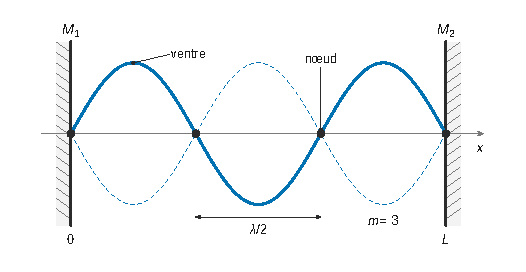
\includegraphics{figures/q19-mode-stationnaire.pdf}
\caption*{Figure 3 --- Mode m = 3 de la cavité sans pertes : un nœud de champ
électrique sur chaque miroir, d'où L = mλ/2}
\end{figure}

\hypertarget{ii-cavituxe9-avec-pertes}{%
\subsection{II --- Cavité avec pertes}\label{ii-cavituxe9-avec-pertes}}

Un miroir laisse fuir la lumière : on calcule l'onde intracavité par superposition d'allers-retours. Outils : coefficients de réflexion et transmission, module d'un complexe, trigonométrie.

\hypertarget{question-20}{%
\subsection{Question 20}\label{question-20}}

\begin{indication}{1}

\(R\) et \(T\) sont des rapports d'intensités, c'est-à-dire de puissances surfaciques.

\end{indication}

\hypertarget{solution-19}{%
\subsubsection{Solution}\label{solution-19}}

\(R+T=1\iff I_r+I_t=I_i\) : \textbf{conservation de l'énergie au niveau du miroir, supposé sans absorption ni diffusion.}

\begin{piege}

Il faut nommer l'hypothèse sous-jacente : un miroir réel absorbe un peu, et l'on a alors \(R+T<1\).

\end{piege}

\hypertarget{question-21}{%
\subsection{Question 21}\label{question-21}}

\begin{indication}{1}

Quelles ondes \emph{arrivent} sur \(M_1\), et de quel côté ? Laquelle en \emph{repart} vers la droite ?

\end{indication}

\hypertarget{solution-20}{%
\subsubsection{Solution}\label{solution-20}}

Juste à droite de \(M_1\), l'onde allant vers la droite est la superposition (linéarité des équations de Maxwell) de deux ondes :

\begin{itemize}
\tightlist
\item
  la partie \textbf{transmise} de l'onde de pompe arrivant par la gauche, \(\tau\underline E_p\) ;
\item
  la partie \textbf{réfléchie} sur la face interne de \(M_1\) de l'onde intracavité revenant de \(M_2\), \(r\underline E_G\) (même \(r\) dans les deux sens).
\end{itemize}

D'où \(\underline E_D=\tau\underline E_p+r\underline E_G\).

\hypertarget{question-22}{%
\subsection{Question 22}\label{question-22}}

\begin{indication}{1}

\(M_2\) est toujours un conducteur parfait : réutilisez la condition de Q18 en \(x=L\).

\end{indication}

\hypertarget{solution-21}{%
\subsubsection{Solution}\label{solution-21}}

Avec le champ \(\left(\underline E_De^{-jkx}+\underline E_Ge^{jkx}\right)e^{j\omega t}\vec u_y\), la condition \(\underline E_De^{-jkL}+\underline E_Ge^{jkL}=0\) donne

\equationajustee{\boxed{\underline E_G=-\underline E_D\,e^{-2jkL}}}

déphasage d'aller-retour \(2kL\) et réflexion de coefficient \(-1\).

\begin{piege}

Deux facteurs à ne pas perdre : \(2kL\) (aller \emph{et} retour) et le signe moins. Une erreur sur l'un ou l'autre déplace les résonances en \(kL=(m+\frac12)\pi\), en contradiction avec Q19.

\end{piege}

\hypertarget{question-23}{%
\subsection{Question 23}\label{question-23}}

\begin{indication}{1}

Reportez Q22 dans la relation de Q21, puis remplacez \(r\) et \(\tau\) par leurs valeurs.

\end{indication}

\hypertarget{solution-22}{%
\subsubsection{Solution}\label{solution-22}}

\(\underline E_D\left(1+re^{-2jkL}\right)=\tau\underline E_p\), et avec \(r=-\sqrt R\), \(\tau=\sqrt{1-R}\) :

\equationajustee{\boxed{\frac{\underline E_D}{\underline E_p}=\frac{\sqrt{1-R}}{1-\sqrt R\,e^{-2jkL}}}}

\hypertarget{question-24}{%
\subsection{Question 24}\label{question-24}}

\begin{indication}{1}

L'intensité est proportionnelle au module carré de l'amplitude, avec le même coefficient pour deux ondes dans le même milieu.

\end{indication}

\begin{indication}{2}

Développez \(\lvert1-\sqrt Re^{-2jkL}\rvert^2\), puis utilisez \(1-\cos2\theta=2\sin^2\theta\).

\end{indication}

\hypertarget{solution-23}{%
\subsubsection{Solution}\label{solution-23}}

\equationajustee{\begin{aligned}
\left\lvert1-\sqrt Re^{-2jkL}\right\rvert^2&=1+R-2\sqrt R\cos2kL\\
&=(1-\sqrt R)^2+4\sqrt R\sin^2kL
\end{aligned}}

\equationajustee{\frac{I_D}{I_p}=\frac{g}{1+\dfrac{4\sqrt R}{(1-\sqrt R)^2}\sin^2kL}}

\equationajustee{\boxed{\begin{aligned}
g&=\frac{1-R}{(1-\sqrt R)^2}\\
&=\frac{1+\sqrt R}{1-\sqrt R}
\end{aligned}}}

Contrôle : \(R=0\) donne \(g=1\) et \(I_D=I_p\).

\hypertarget{question-25}{%
\subsection{Question 25}\label{question-25}}

\begin{indication}{1}

Chiffrez le coefficient devant \(\sin^2kL\) pour \(R=0{,}960\).

\end{indication}

\begin{indication}{2}

Comparez la valeur du rapport en \(\sin kL=0\) et pour \(\sin kL\) de l'ordre de 1.

\end{indication}

\hypertarget{solution-24}{%
\subsubsection{Solution}\label{solution-24}}

\equationajustee{\begin{aligned}
\sqrt R&=0{,}9798\\
g&\approx98\\
\mathcal M&=4\sqrt R/(1-\sqrt R)^2\\
&\approx9{,}6\times10^3
\end{aligned}}

Le rapport vaut 98 pour \(\sin kL=0\). Il tombe sous \(g/2\) dès que \(\lvert\sin kL\rvert>1/\sqrt{\mathcal M}\approx10^{-2}\). Il atteint au minimum \(g/(1+\mathcal M)\approx10^{-2}\) : il est négligeable devant son maximum sauf au voisinage immédiat de

\equationajustee{\boxed{k=\frac{m\pi}{L},\ m\in\mathbb N^*}}

\begin{methode}

« Quasiment nul » se démontre par un ordre de grandeur chiffré, ici \(\mathcal M\sim10^4\).

\end{methode}

\hypertarget{question-26}{%
\subsection{Question 26}\label{question-26}}

\begin{indication}{1}

Période en \(kL\), position, hauteur et largeur des pics : tout est déjà calculé ou presque.

\end{indication}

\hypertarget{solution-25}{%
\subsubsection{Solution}\label{solution-25}}

Courbe \(\pi\)-périodique en \(kL\) : pics de hauteur \(g\approx98\) en \(kL=m\pi\).

Leur largeur à mi-hauteur vaut \(2/\sqrt{\mathcal M}\approx2\times10^{-2}\) rad (0,65 \% de la période).

Entre les pics, fond quasi nul de minimum \(\approx10^{-2}\) en \(kL=\pi/2+m\pi\).

\begin{figure}[H]
\centering
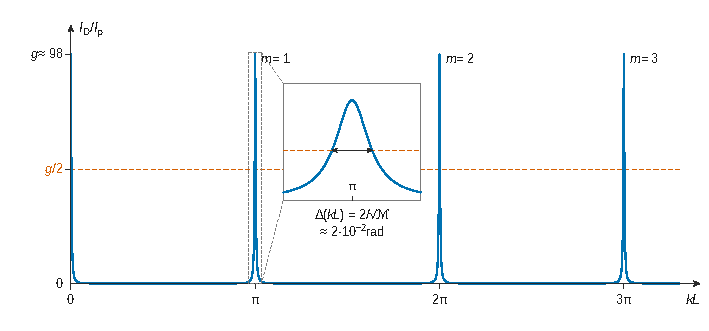
\includegraphics{figures/q26-fonction-airy.pdf}
\caption*{Figure 4 --- Rapport I\_D/I\_p en fonction de kL pour R = 96 \% : pics
de hauteur g ≈ 98 en kL = mπ, de largeur à mi-hauteur 2/√ℳ ≈ 2·10⁻² rad
(zoom), fond quasi nul}
\end{figure}

\begin{piege}

La période est \(\pi\) (et non \(2\pi\)), car seul \(\sin^2kL\) intervient. Des pics dessinés larges trahissent l'oubli de \(\mathcal M\sim10^4\).

\end{piege}

\hypertarget{question-27}{%
\subsection{Question 27}\label{question-27}}

\begin{indication}{1}

Traduisez la condition de maximum en fréquence avec la relation de dispersion.

\end{indication}

\hypertarget{solution-26}{%
\subsubsection{Solution}\label{solution-26}}

\(k_m=m\pi/L\), d'où

\equationajustee{\boxed{\begin{aligned}
\nu_m&=m\frac{c}{2L}\\
\mathrm{FSR}'_\nu&=\frac{c}{2L}\\
&={\mathrm{FSR}}_\nu
\end{aligned}}}

Mêmes fréquences de modes et même intervalle spectral libre que sans pertes. Mais les modes ne sont plus des fréquences isolées : ce sont des résonances de largeur finie \(\Delta\nu_c\), toute fréquence pénétrant un peu dans la cavité.

\hypertarget{question-28}{%
\subsection{Question 28}\label{question-28}}

\begin{indication}{1}

Écrivez la condition de mi-hauteur, puis linéarisez \(\sin kL\) près d'un maximum.

\end{indication}

\begin{indication}{2}

\(kL\) est proportionnel à \(\nu\) : la largeur en \(kL\) se convertit directement en largeur en fréquence.

\end{indication}

\hypertarget{solution-27}{%
\subsubsection{Solution}\label{solution-27}}

Mi-hauteur : \(\mathcal M\sin^2kL=1\). Près de \(kL=m\pi\), comme \(1/\sqrt{\mathcal M}\ll1\), on trouve \(\delta_{1/2}=\pm1/\sqrt{\mathcal M}\).

Donc \(\Delta(kL)=2/\sqrt{\mathcal M}\). Comme \(kL=\pi\nu/\mathrm{FSR}'_\nu\) :

\equationajustee{\boxed{\begin{aligned}
\mathcal F&=\frac{\pi}{\Delta(kL)}\\
&=\frac{\pi\sqrt{\mathcal M}}{2}\\
&=\frac{\pi R^{1/4}}{1-\sqrt R}
\end{aligned}}}

Application numérique :

\equationajustee{\boxed{\mathcal F\approx154}}

\begin{methode}

La finesse d'une cavité de type Fabry-Pérot ne dépend que des réflectivités ; elle compte, à un facteur près, le nombre d'allers-retours de la lumière avant sa sortie.

\end{methode}

\hypertarget{question-29}{%
\subsection{Question 29}\label{question-29}}

\begin{indication}{1}

Finesse, largeur spectrale, temps de cohérence : enchaînez.

\end{indication}

\hypertarget{solution-28}{%
\subsubsection{Solution}\label{solution-28}}

Une grande finesse donne une raie fine, \(\Delta\nu_c={\mathrm{FSR}}_\nu/\mathcal F\). Elle donne donc une \textbf{grande longueur de cohérence} \(\ell_c\approx c/\Delta\nu_c=2L\mathcal F\). Les interférences restent alors observables pour de grandes différences de marche, d'où des mesures interférométriques très sensibles (petits déplacements, métrologie).

\begin{piege}

« La raie est plus fine » ne suffit pas : il faut aller jusqu'à la différence de marche accessible.

\end{piege}

\begin{center}\rule{0.5\linewidth}{0.5pt}\end{center}

\hypertarget{partie-c-milieu-amplificateur-dun-laser}{%
\section{Partie C --- Milieu amplificateur d'un laser}\label{partie-c-milieu-amplificateur-dun-laser}}

\hypertarget{i-uxe9volution-de-populations}{%
\subsection{I --- Évolution de populations}\label{i-uxe9volution-de-populations}}

Le milieu est décrit comme un réseau de réactions d'ordre 1. Outils : cinétique chimique, régime stationnaire, étude de signe.

\hypertarget{question-30}{%
\subsection{Question 30}\label{question-30}}

\begin{indication}{1}

Pour une réaction d'ordre 1, la vitesse est la constante de vitesse multipliée par la concentration de l'espèce qui disparaît.

\end{indication}

\hypertarget{solution-29}{%
\subsubsection{Solution}\label{solution-29}}

\equationajustee{\boxed{\begin{aligned}
v_{\mathrm{pomp}}&=\Gamma n_1\\
v_{\mathrm{nr}}&=k_{\mathrm{nr}}n_3\\
v_{\mathrm{abs}}&=\beta n_1\\
v_{\mathrm{stim}}&=\beta n_2\\
v_{\mathrm{spont}}&=An_2
\end{aligned}}}

\hypertarget{question-31}{%
\subsection{Question 31}\label{question-31}}

\begin{indication}{1}

Recensez les processus qui créent ou détruisent M (état fondamental), avec leur signe.

\end{indication}

\hypertarget{solution-30}{%
\subsubsection{Solution}\label{solution-30}}

M est consommé par le pompage (\(-\Gamma n_1\)) et l'absorption (\(-\beta n_1\)). Il est produit par les émissions spontanée (\(+An_2\)) et stimulée (\(+\beta n_2\)) ; la désexcitation non radiative ne le concerne pas. D'où

\equationajustee{\frac{\mathrm dn_1}{\mathrm dt}=-\Gamma n_1+An_2+\beta n_2-\beta n_1}

\hypertarget{question-32}{%
\subsection{Question 32}\label{question-32}}

\begin{indication}{1}

Même recensement pour M* et M**, en suivant les flèches de la figure 5.

\end{indication}

\hypertarget{solution-31}{%
\subsubsection{Solution}\label{solution-31}}

\equationajustee{\boxed{\begin{aligned}
\frac{\mathrm dn_2}{\mathrm dt}&=k_{\mathrm{nr}}n_3+\beta n_1-\beta n_2-An_2\\
\frac{\mathrm dn_3}{\mathrm dt}&=\Gamma n_1-k_{\mathrm{nr}}n_3
\end{aligned}}}

\begin{piege}

Le pompage relie M à M** sans passer par M* : \(\Gamma\) n'apparaît pas dans \(\mathrm dn_2/\mathrm dt\).

\end{piege}

\hypertarget{question-33}{%
\subsection{Question 33}\label{question-33}}

\begin{indication}{1}

Additionnez les trois équations.

\end{indication}

\hypertarget{solution-32}{%
\subsubsection{Solution}\label{solution-32}}

La somme est nulle, donc \textbf{\(n_1+n_2+n_3\) est constant} : les processus redistribuent l'espèce M entre ses niveaux sans en créer ni en détruire (conservation de la matière).

\hypertarget{question-34}{%
\subsection{Question 34}\label{question-34}}

\begin{indication}{1}

En régime stationnaire, commencez par l'équation la plus simple, celle de \(n_3\).

\end{indication}

\begin{indication}{2}

Exprimez \(n_1\) puis \(n_2\) en fonction de \(n_3\) ; l'une des trois équations est redondante.

\end{indication}

\hypertarget{solution-33}{%
\subsubsection{Solution}\label{solution-33}}

\(n_1=\dfrac{k_{\mathrm{nr}}}{\Gamma}n_3\) ; puis \(k_{\mathrm{nr}}n_3+\beta n_1=(A+\beta)n_2\) donne \((\Gamma+\beta)n_1=(A+\beta)n_2\). Donc

\equationajustee{\boxed{\begin{aligned}
\Delta n&=n_2-n_1\\
&=\frac{k_{\mathrm{nr}}(\Gamma-A)}{\Gamma(A+\beta)}\,n_3
\end{aligned}}}

\begin{methode}

Une loi de conservation rend le système stationnaire de rang inférieur au nombre d'inconnues : ne cherchez pas d'équation supplémentaire.

\end{methode}

\hypertarget{question-35}{%
\subsection{Question 35}\label{question-35}}

\begin{indication}{1}

Étudiez le signe de chaque facteur de l'expression de Q34.

\end{indication}

\hypertarget{solution-34}{%
\subsubsection{Solution}\label{solution-34}}

Tous les facteurs sont positifs sauf \(\Gamma-A\) :

\equationajustee{\boxed{\Delta n>0\iff\Gamma>A}}

Le pompage doit alimenter le niveau excité (via M**, vidé très vite) plus vite que l'émission spontanée ne le vide.

\hypertarget{ii-bilan-de-puissance-uxe9lectromagnuxe9tique-dans-le-milieu-amplificateur}{%
\subsection{II --- Bilan de puissance électromagnétique dans le milieu amplificateur}\label{ii-bilan-de-puissance-uxe9lectromagnuxe9tique-dans-le-milieu-amplificateur}}

On passe des populations à l'onde : un bilan local fait apparaître un gain linéique. Outils : bilan d'énergie sur une tranche, vecteur de Poynting, équation différentielle du premier ordre.

\hypertarget{question-36}{%
\subsection{Question 36}\label{question-36}}

\begin{indication}{1}

Pour chaque processus : un photon de l'onde laser (direction, fréquence, phase) est-il créé, détruit, ou rien de tout cela ?

\end{indication}

\hypertarget{solution-35}{%
\subsubsection{Solution}\label{solution-35}}

\begin{itemize}
\tightlist
\item
  pompage : énergie extérieure, autre fréquence ; \textbf{pas de contribution directe} ;
\item
  non radiatif : pas de photon ; \textbf{pas de contribution} ;
\item
  absorption : un photon \(\hbar\omega\) retiré à l'onde, \textbf{perte} ;
\item
  émission stimulée : un photon cohérent ajouté, \textbf{gain} ;
\item
  émission spontanée : photon isotrope et incohérent, hors du faisceau ; énergie \textbf{perdue pour l'onde laser}.
\end{itemize}

\begin{piege}

L'émission spontanée produit bien des photons, mais pas dans le mode laser : elle ne compte pas comme un gain.

\end{piege}

\hypertarget{question-37}{%
\subsection{Question 37}\label{question-37}}

\begin{indication}{1}

Système : tranche \([x,x+\mathrm dx]\) de section \(S\), durée \(\mathrm dt\). Variation d'énergie = flux entrant net + termes d'échange avec la matière.

\end{indication}

\begin{indication}{2}

Chaque événement échange \(\hbar\omega\) ; remplacez ensuite \(u_{\text{\text{ém}}}\) par \(\Pi/c\), y compris dans \(\beta=bu_{\text{\text{ém}}}\).

\end{indication}

\hypertarget{solution-36}{%
\subsubsection{Solution}\label{solution-36}}

\equationajustee{\frac{\partial u_{\text{\text{ém}}}}{\partial t}=-\frac{\partial\Pi}{\partial x}+\hbar\omega\beta(n_2-n_1)-\hbar\omega An_2}

Avec \(u_{\text{\text{ém}}}=\Pi/c\) et \(\beta=b\Pi/c\) :

\equationajustee{\boxed{\frac{\partial\Pi}{\partial x}+\frac1c\frac{\partial\Pi}{\partial t}=\gamma\Pi-p}}

\equationajustee{\boxed{\begin{aligned}
\gamma(\omega)&=\frac{b\hbar\omega(n_2-n_1)}{c}\\
p(\omega)&=\hbar\omega An_2
\end{aligned}}}

\(\gamma\) est en m⁻¹, \(p\) en W·m⁻³.

\begin{methode}

Un bilan local se pose toujours ainsi : système défini, durée \(\mathrm dt\), chaque terme avec son signe, puis division par \(S\,\mathrm dx\,\mathrm dt\) et contrôle d'homogénéité.

\end{methode}

\begin{piege}

Le signe de \(p\) est imposé par la forme de l'énoncé : l'émission spontanée y est traitée comme une perte pour le faisceau. C'est une convention de modélisation, sans effet sur la suite puisque \(p\) est négligé dès Q38.

\end{piege}

\hypertarget{question-38}{%
\subsection{Question 38}\label{question-38}}

\begin{indication}{1}

Réécrivez \(\gamma\Pi\) et \(p\) en vitesses de processus.

\end{indication}

\hypertarget{solution-37}{%
\subsubsection{Solution}\label{solution-37}}

\(\gamma\Pi=\hbar\omega\beta\Delta n\) et \(p=\hbar\omega An_2\) : la condition équivaut à \(An_2\ll\beta\Delta n\). \textbf{L'émission spontanée, incohérente, est négligeable devant l'émission stimulée nette, cohérente} : la lumière produite est directive, monochromatique et cohérente, c'est-à-dire une lumière laser.

\hypertarget{question-39}{%
\subsection{Question 39}\label{question-39}}

\begin{indication}{1}

En régime stationnaire, l'équation devient différentielle ordinaire en \(x\), linéaire à coefficients constants.

\end{indication}

\hypertarget{solution-38}{%
\subsubsection{Solution}\label{solution-38}}

\(\dfrac{\mathrm d\Pi}{\mathrm dx}=\gamma\Pi-p\) et \(\Pi(0)=\Pi_0\) donnent

\equationajustee{\Pi(x)=\left(\Pi_0-\frac p\gamma\right)e^{\gamma x}+\frac p\gamma}

soit, avec \(p\ll\gamma\Pi\),

\equationajustee{\boxed{\Pi(x)=\Pi_0e^{\gamma x}}}

\hypertarget{question-40}{%
\subsection{Question 40}\label{question-40}}

\begin{indication}{1}

Quelle est la dimension de \(\gamma\) ? Que représente \(\frac1\Pi\frac{\mathrm d\Pi}{\mathrm dx}\) ?

\end{indication}

\hypertarget{solution-39}{%
\subsubsection{Solution}\label{solution-39}}

\(\gamma\) est le \textbf{gain linéique} (m⁻¹) : l'intensité varie d'un facteur \(e\) sur \(1/\lvert\gamma\rvert\). Son signe est celui de \(\Delta n\) :

\begin{itemize}
\tightlist
\item
  amplification si \(\Delta n>0\) ;
\item
  atténuation (Beer-Lambert) si \(\Delta n<0\) ;
\item
  transparence si \(\Delta n=0\).
\end{itemize}

En régime stationnaire :

\equationajustee{\boxed{\gamma>0\iff\Delta n>0\iff\Gamma>A}}

\begin{methode}

Un milieu ordinaire (\(\Delta n<0\)) absorbe : c'est la loi de Beer-Lambert. L'effet laser commence par l'inversion de ce signe.

\end{methode}

\hypertarget{iii-considuxe9rations-expuxe9rimentales-pour-un-laser-uxe0-colorant-compact}{%
\subsection{III --- Considérations expérimentales pour un laser à colorant compact}\label{iii-considuxe9rations-expuxe9rimentales-pour-un-laser-uxe0-colorant-compact}}

On applique les résultats de la partie B à un spectre réel. Outils : lecture de figure, différentiation, ordres de grandeur.

\hypertarget{question-41}{%
\subsection{Question 41}\label{question-41}}

\begin{indication}{1}

Une solution colorée apparaît de la couleur complémentaire de celle qu'elle absorbe.

\end{indication}

\hypertarget{solution-40}{%
\subsubsection{Solution}\label{solution-40}}

La solution absorbe entre 550 et 620 nm (vert-jaune-orangé) et apparaît de la couleur complémentaire, \textbf{bleue}. L'émission laser, entre 687 et 704 nm (figure 6), est \textbf{rouge profond}, à la limite du proche infrarouge.

\begin{piege}

Un colorant « bleu » n'absorbe pas le bleu : il le transmet.

\end{piege}

\hypertarget{question-42}{%
\subsection{Question 42}\label{question-42}}

\begin{indication}{1}

Refaites Q19 dans un milieu d'indice \(n\) : la célérité devient \(c/n\).

\end{indication}

\begin{indication}{2}

Exprimez la longueur d'onde (dans le vide) du mode \(m\), puis l'écart entre deux modes voisins, sachant que \(m\gg1\).

\end{indication}

\hypertarget{solution-41}{%
\subsubsection{Solution}\label{solution-41}}

\(k=n\omega/c\) et \(kL=m\pi\) donnent

\equationajustee{\begin{aligned}
\nu_m&=\frac{mc}{2nL}\\
{\mathrm{FSR}}_\nu&=\frac{c}{2nL}
\end{aligned}}

Avec \(\lambda_m=c/\nu_m=2nL/m\) :

\equationajustee{\begin{aligned}
{\mathrm{FSR}}_\lambda&=\lambda_m-\lambda_{m+1}\\
&=\frac{2nL}{m(m+1)}\\
&\approx\frac{\lambda^2}{2nL}\qquad(m\approx650)
\end{aligned}}

\begin{methode}

Conversion d'un petit écart : \(\lvert\mathrm d\lambda\rvert=\dfrac{\lambda^2}{c}\lvert\mathrm d\nu\rvert\).

\end{methode}

\hypertarget{question-43}{%
\subsection{Question 43}\label{question-43}}

\begin{indication}{1}

Mesurez l'intervalle spectral libre sur le plus grand nombre possible d'intervalles, puis inversez la formule de Q42.

\end{indication}

\begin{indication}{2}

Contrôle gratuit : les numéros de mode sont écrits sur la figure.

\end{indication}

\hypertarget{solution-42}{%
\subsubsection{Solution}\label{solution-42}}

Les pics vont du mode 664 (\(\approx687{,}7\) nm) au mode 649 (\(\approx703{,}7\) nm). On en tire \({\mathrm{FSR}}_\lambda\approx16{,}0/15\approx1{,}06\) nm (insert : 1,02 à 1,08 nm).

\equationajustee{\begin{aligned}
L&=\frac{\lambda^2}{2n\,{\mathrm{FSR}}_\lambda}\\
&=\frac{(695\times10^{-9})^2}{2\times1{,}3587\times1{,}06\times10^{-9}}
\end{aligned}}

\equationajustee{\boxed{L\approx1{,}7\times10^{-4}\ \mathrm m}}

Contrôle : \(L=m\lambda_m/(2n)=657\times695\ \mathrm{nm}/(2\times1{,}3587)=0{,}168\) mm.

\begin{piege}

Oublier l'indice surestime \(L\) de 36 \%, ce que contredit la numérotation des modes.

\end{piege}

\hypertarget{question-44}{%
\subsection{Question 44}\label{question-44}}

\begin{indication}{1}

Différentiez \(\nu=c/\lambda\) et remarquez que le même facteur intervient au numérateur et au dénominateur de la finesse.

\end{indication}

\hypertarget{solution-43}{%
\subsubsection{Solution}\label{solution-43}}

\(\lvert\Delta\nu\rvert=\dfrac{c}{\lambda^2}\lvert\Delta\lambda\rvert\) pour \(\Delta\lambda\ll\lambda\), avec le même facteur pour \(\mathrm{FSR}\) et \(\Delta\nu_c\) pris à la même longueur d'onde :

\equationajustee{\boxed{\mathcal F=\frac{{\mathrm{FSR}}_\lambda}{\Delta\lambda_c}}}

Application numérique : \(\mathcal F\approx1{,}06/0{,}1\), soit

\equationajustee{\boxed{\mathcal F\sim10}}

\begin{piege}

L'énoncé demande un ordre de grandeur : \(\Delta\lambda_c\) n'est connu qu'« environ », annoncer trois chiffres significatifs serait une fausse précision.

\end{piege}

\hypertarget{question-45}{%
\subsection{Question 45}\label{question-45}}

\begin{indication}{1}

Dans \(\lambda_m=2nL/m\), quelles grandeurs sont fixées par construction ?

\end{indication}

\hypertarget{solution-44}{%
\subsubsection{Solution}\label{solution-44}}

\(m\) est entier et \(L\) géométrique : le paramètre sensible est \textbf{l'indice \(n\) de la solution}, qui dépend de la température et de la composition.

On le suit par le déplacement des pics, \(\delta\lambda_m/\lambda_m=\delta n/n\).

\begin{piege}

« La longueur d'onde » est l'observable mesurée ; le \emph{paramètre} sensible demandé est l'indice.

\end{piege}

\hypertarget{question-46}{%
\subsection{Question 46}\label{question-46}}

\begin{indication}{1}

Question à initiative. Listez ce qui change (\(L\)) et ce qui ne change pas (miroirs, donc finesse ; colorant, donc bande de gain).

\end{indication}

\begin{indication}{2}

Chiffrez le nouvel intervalle spectral libre pour \(L\approx1\) m et comparez-le à la largeur de la bande de gain et à la résolution d'un spectromètre.

\end{indication}

\begin{indication}{3}

Dessinez deux spectres côte à côte, à la même échelle en longueur d'onde.

\end{indication}

\hypertarget{solution-45}{%
\subsubsection{Solution}\label{solution-45}}

\emph{Hypothèses.} Finesse \(\approx10\) inchangée, bande de gain inchangée (environ 687--704 nm), \(L\) multiplié par environ \(6\times10^3\).

\emph{Chiffrage.} Avec \(n=1{,}3587\) :

\equationajustee{\begin{aligned}
{\mathrm{FSR}}_\lambda&=\frac{(695\times10^{-9})^2}{2\times1{,}3587\times1}\\
&=1{,}8\times10^{-4}\ \mathrm{nm}
\end{aligned}}

\equationajustee{\begin{aligned}
{\mathrm{FSR}}_\nu&=\frac{c}{2nL}\\
&=110\ \mathrm{MHz}
\end{aligned}}

(\(2{,}4\times10^{-4}\) nm si la cavité est essentiellement dans l'air.) La bande de gain contient \(N\approx15\text{–}20\ \mathrm{nm}/1{,}8\times10^{-4}\ \mathrm{nm}\sim10^5\) modes, chacun de largeur \(\approx2\times10^{-5}\) nm.

\emph{Allure.} Un spectromètre usuel (\(10^{-2}\) à \(10^{-1}\) nm) ne sépare pas des modes 50 à 500 fois plus serrés que sa résolution : le spectre observé est une \textbf{bande quasi continue} épousant la courbe de gain du colorant, au lieu du peigne de seize pics de la figure 6.

\begin{figure}[H]
\centering
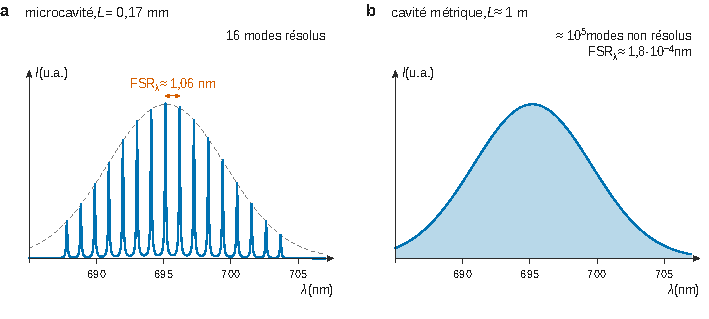
\includegraphics{figures/q46-spectres-cavite-courte-longue.pdf}
\caption*{Figure 5 --- Allure des spectres à colorant et miroirs identiques : (a)
microcavité, 16 modes séparés de 1,06 nm ; (b) cavité métrique, environ
10⁵ modes non résolus, bande continue sous la courbe de gain}
\end{figure}

\emph{Commentaire.} Plus la cavité est courte, plus les modes sont espacés : la microcavité sélectionne naturellement une quinzaine de modes séparés, ce qui en fait un capteur. Le laser à cavité métrique est fortement multimode (la compétition entre modes limite le nombre de modes oscillants sans rendre le spectre résoluble) ; pour le rendre monomode et accordable, on ajoute des éléments sélectifs (réseau, étalon, filtre biréfringent). En échange, il offre un grand volume de milieu amplificateur et davantage de puissance.

\begin{jury}

Sur une question ouverte de fin de sujet, un raisonnement qualitatif ne suffit pas : on attend des hypothèses explicites, un chiffrage (ici l'intervalle spectral libre et le nombre de modes), un schéma légendé et un commentaire physique.

\end{jury}

\begin{center}\rule{0.5\linewidth}{0.5pt}\end{center}

\hypertarget{bilan}{%
\section{Bilan}\label{bilan}}

\textbf{Méthodes à retenir.}

\begin{itemize}
\tightlist
\item
  Minorer une énergie quantique avec l'inégalité de Heisenberg, puis minimiser (\(a/X+bX\ge2\sqrt{ab}\)).
\item
  Adimensionner une équation de Schrödinger et quantifier par le monôme dominant d'une solution polynomiale.
\item
  Lire un spectre rovibrationnel : trou central (\(\Delta J=0\) interdit), branches P et R, attribution à partir du centre, extinction thermique.
\item
  Extraire deux paramètres de deux mesures par somme et différence, propager les incertitudes-types (facteur \(\frac{\sqrt2}{2}\) ; exposant pour une puissance).
\item
  Construire l'onde intracavité d'un Fabry-Pérot par superposition, en suivant signes et déphasage d'aller-retour ; finesse \(\mathcal F=\pi R^{1/4}/(1-\sqrt R)\).
\item
  Poser un bilan local d'énergie électromagnétique avec terme source.
\item
  Passer d'un écart en fréquence à un écart en longueur d'onde : \(\lvert\Delta\lambda\rvert=\lambda^2\lvert\Delta\nu\rvert/c\).
\end{itemize}

\textbf{Prérequis à revoir.} Inégalité de Heisenberg et états stationnaires ; relations de passage et conducteur parfait ; ondes stationnaires dans une cavité ; cohérence temporelle ; cinétique d'ordre 1 et approximation des régimes stationnaires ; couleurs complémentaires.

\textbf{Questions classiques transposables.} Énergie de point zéro par Heisenberg (oscillateur, puits infini, atome d'hydrogène) ; modes d'une corde vibrante ou d'un tuyau sonore (même condition \(kL=m\pi\)) ; interféromètre de Fabry-Pérot en optique ; laser à trois ou quatre niveaux ; loi de Beer-Lambert en chimie analytique ; effet isotopique sur une fréquence de vibration (spectroscopie infrarouge de chimie organique, liaisons C--H et C--D).

\end{document}
